\documentclass[UTF8,a4paper,zihao=-4]{ctexart}

\usepackage{geometry}
\usepackage{amsmath,amssymb,amsfonts}
\usepackage{newtxmath}
\usepackage{booktabs}
\usepackage{graphicx}
\usepackage{float}
\usepackage{caption}
\usepackage{subcaption}
\usepackage{enumitem}
\usepackage{setspace}
\usepackage[numbers,sort&compress]{natbib}
\usepackage{hyperref}
\usepackage{fancyhdr}

\geometry{top=2.5cm,bottom=2.5cm,left=2.5cm,right=2.5cm}
\graphicspath{{figures/}}
\setstretch{1.0}
\setlength{\parindent}{2em}
\setlength{\parskip}{3pt plus 1pt minus 1pt}
\setlength{\intextsep}{8pt plus 1pt minus 1pt}
\setlength{\textfloatsep}{8pt plus 1pt minus 1pt}
\setlength{\floatsep}{8pt plus 1pt minus 1pt}
\setlength{\abovedisplayskip}{0.6em plus 0.2em minus 0.1em}
\setlength{\belowdisplayskip}{0.6em plus 0.2em minus 0.1em}
\setlength{\abovedisplayshortskip}{0.35em plus 0.15em minus 0.1em}
\setlength{\belowdisplayshortskip}{0.35em plus 0.15em minus 0.1em}

\newcommand{\sectiontitlefont}{\heiti\fontsize{18bp}{25bp}\selectfont}
\newcommand{\subsectiontitlefont}{\heiti\fontsize{14bp}{20bp}\selectfont}
\newcommand{\subsubsectiontitlefont}{\heiti\fontsize{12bp}{17bp}\selectfont}
\newcommand{\paragraphtitlefont}{\heiti\fontsize{12bp}{17bp}\selectfont}

\hypersetup{
  colorlinks=true,
  linkcolor=black,
  citecolor=black,
  urlcolor=black
}

\ctexset{
  section = {
    format = \centering\sectiontitlefont,
    nameformat = \sectiontitlefont,
    numberformat = \sectiontitlefont,
    titleformat = \sectiontitlefont,
    name = {},
    number = \chinese{section},
    aftername = \quad,
    beforeskip = 22pt plus 2pt minus 2pt,
    afterskip = 14pt plus 1pt minus 1pt
  },
  subsection = {
    format = \raggedright\subsectiontitlefont,
    nameformat = \subsectiontitlefont,
    numberformat = \subsectiontitlefont,
    titleformat = \subsectiontitlefont,
    name = {},
    number = \arabic{section}.\arabic{subsection},
    aftername = \quad,
    beforeskip = 12pt plus 1pt minus 1pt,
    afterskip = 6pt plus 1pt minus 1pt
  },
  subsubsection = {
    format = \raggedright\subsubsectiontitlefont,
    nameformat = \subsubsectiontitlefont,
    numberformat = \subsubsectiontitlefont,
    titleformat = \subsubsectiontitlefont,
    name = {},
    number = \arabic{section}.\arabic{subsection}.\arabic{subsubsection},
    aftername = \quad,
    beforeskip = 8pt plus 1pt minus 1pt,
    afterskip = 4pt plus 1pt minus 1pt
  },
  paragraph = {
    format = \raggedright\paragraphtitlefont,
    nameformat = \paragraphtitlefont,
    titleformat = \paragraphtitlefont,
    name = {},
    number = {},
    aftername = {},
    beforeskip = 6pt,
    afterskip = 3pt
  }
}

\DeclareCaptionFont{captionkai}{\kaishu\zihao{-4}\setstretch{1.0}}
\DeclareCaptionLabelFormat{tablecn}{表\thetable}
\DeclareCaptionLabelFormat{figurecn}{图\thefigure}
\captionsetup{
  font = captionkai,
  labelfont = captionkai,
  labelsep = quad,
  justification = centering
}
\captionsetup[figure]{
  name = 图,
  labelformat = figurecn,
  position = bottom,
  skip = 6pt,
  belowskip = 8pt
}
\captionsetup[table]{
  name = 表,
  labelformat = tablecn,
  position = top,
  skip = 6pt,
  belowskip = 8pt
}

\renewcommand{\bibsection}{\section*{参考文献}}
\bibliographystyle{unsrtnat}

\newcommand{\tablefont}{\songti\zihao{-4}}
\newcommand{\tablehead}[1]{\heiti\zihao{-4}#1}

\pagestyle{fancy}
\fancyhf{}
\fancyfoot[C]{\thepage}
\renewcommand{\headrulewidth}{0pt}

\newcommand{\paperTitle}{绿电直连型电氢氨园区优化运行}
\newcommand{\registrationLabel}{参赛编号}
\newcommand{\paperTitleLabel}{论文题目}
\newcommand{\registrationNumber}{009842}

\begin{document}

\begin{titlepage}
  \thispagestyle{empty}
  \centering
  \vspace*{8.5cm}
  {\heiti\zihao{2} \registrationLabel：\registrationNumber\par}
  \vspace{3cm}
  {\heiti\zihao{2} \paperTitleLabel：\paperTitle\par}
  \vfill
\end{titlepage}

\clearpage
\setcounter{page}{1}
\pagestyle{fancy}

\begin{center}
  {\heiti\zihao{3}\paperTitle}
\end{center}

\noindent{\heiti 摘要：}
本文围绕题目给定问题，首先对数据和约束条件进行整理，随后建立相应的数学模型，并通过算法求解得到主要结论。
摘要应简明扼要说明研究问题、建模方法、求解过程和核心结果，篇幅控制在一页以内。

\vspace{1em}
\noindent{\heiti 关键词：}
关键词一；关键词二；关键词三；数学建模


\clearpage
\section{问题重述}

本节对竞赛题目中的实际背景、研究对象、已知条件和需要解决的问题进行准确转述。
写作时应避免加入队员、学校等身份信息。

\subsection{问题背景}

概述题目背景及其工程或管理意义。

\subsection{待解决问题}

将题目要求拆解为若干可建模、可计算、可验证的子问题。

\section{问题分析}

本节分析各子问题的主要影响因素、变量关系、约束条件和求解难点，为模型建立提供依据。

\section{模型假设}

为便于建模，作出如下合理假设：

\begin{enumerate}[label=\arabic*.]
  \item 假设题目所给数据真实、可靠，且能反映研究对象的主要特征。
  \item 假设未明确给出的外部因素在研究周期内保持稳定。
  \item 假设模型中忽略的次要因素不会显著改变最终结论。
\end{enumerate}

\section{符号说明}

\begin{table}[H]
  \centering
  \caption{主要符号说明}
  \begin{tabular}{cl}
    \toprule
    符号 & 含义 \\
    \midrule
    $x_i$ & 第 $i$ 个决策变量 \\
    $f(x)$ & 目标函数 \\
    $C$ & 约束集合 \\
    \bottomrule
  \end{tabular}
\end{table}

\section{问题一：典型风光场景下运行指标核算}

\subsection{模型建立}

问题一要求在典型风光场景下核算园区固定运行方案的功率曲线、绿电
直连指标与吨氨成本。设第 $t \in \{1,2,\dots,24\}$ 个时段园区新能源
出力、内部用电、网购功率与上网功率分别为
$P_t^{\mathrm{re}}$、$P_t^{\mathrm{use}}$、$P_t^{\mathrm{buy}}$
和 $P_t^{\mathrm{sell}}$。忽略园区功率损耗后，电气节点满足
\begin{equation}
  P^{\mathrm{re}}_t + P^{\mathrm{buy}}_t \;=\; P^{\mathrm{use}}_t + P^{\mathrm{sell}}_t,
  \qquad P^{\mathrm{buy}}_t \cdot P^{\mathrm{sell}}_t = 0,
  \label{eq:power-balance}
\end{equation}
式~\eqref{eq:power-balance} 表示任一时段内园区供给侧与消纳侧的功率
守恒。其中 $P^{\mathrm{re}}_t = P^{\mathrm{wind}}_t + P^{\mathrm{pv}}_t$
为新能源总发电功率，
$P^{\mathrm{use}}_t = P^{\mathrm{ALK}}_t + P^{\mathrm{PEM}}_t
+ P^{\mathrm{NH_3}}_t + P^{\mathrm{load}}_t$ 为园区内部用电功率。
风、光与常规负荷功率均由设备额定容量和附件给定的标幺曲线相乘得到。

问题一中电解槽与合成氨装置均按满负荷连续运行，园区负荷侧功率已知，
故网购功率与上网功率可由每一时段的功率缺额直接确定：
\begin{equation}
  P_t^{\mathrm{buy}}
  = \max\!\left\{P_t^{\mathrm{use}}-P_t^{\mathrm{re}},0\right\},
  \qquad
  P_t^{\mathrm{sell}}
  = \max\!\left\{P_t^{\mathrm{re}}-P_t^{\mathrm{use}},0\right\}.
  \label{eq:p1-grid-exchange}
\end{equation}
式~\eqref{eq:p1-grid-exchange} 将新能源余量映射为上网功率，将功率
缺额映射为网购功率。因此，本问题不涉及生产时段选择与功率调节，
而是以固定负荷方案作为后续优化问题的基线场景。

新能源自发自用电量记为
$E^{\mathrm{self}} = E^{\mathrm{re}} - E^{\mathrm{sell}}$。因此可以得到总用电量为
$E^{\mathrm{total}} = E^{\mathrm{re}} + E^{\mathrm{buy}}
= E^{\mathrm{self}} + E^{\mathrm{sell}} + E^{\mathrm{buy}}$。
三项绿电直连指标分别刻画新能源就地消纳程度、园区用电绿电占比和
新能源余电上网比例，其计算式为:
\begin{align}
  \Pi_{\mathrm{self}}
  &= \frac{E^{\mathrm{self}}}{E^{\mathrm{re}}}, &
  \Pi_{\mathrm{green}}
  &= \frac{E^{\mathrm{self}}}{E^{\mathrm{total}}}, &
  \Pi_{\mathrm{sell}}
  &= \frac{E^{\mathrm{sell}}}{E^{\mathrm{re}}}.
  \label{eq:indicators}
\end{align}
式~\eqref{eq:indicators} 分别反映新能源就地消纳、园区绿电使用程度
和对公共电网反送电的约束。其中三项指标需要分别满足
$\Pi_{\mathrm{self}} > 60\%$、$\Pi_{\mathrm{green}} > 30\%$、
$\Pi_{\mathrm{sell}} < 20\%$。

为进一步评价固定运行方案的经济性，将风电、光伏度电平准化成本，
电氢氨装备运维费用，分时购电费用以及余电上网收入统一计入日运行
成本；日运行成本除以当日制氨量即为吨氨成本：
\begin{equation}
  C^{\mathrm{NH_3}}
  = \frac{
        c^{\mathrm{wind}} E^{\mathrm{wind}}
      + c^{\mathrm{pv}} E^{\mathrm{pv}}
      + \sum\limits_{i\in\mathcal{D}} \mathrm{OPEX}^{i} E^{i}
      + \sum\limits_{t=1}^{24} c^{\mathrm{buy}}_t P^{\mathrm{buy}}_t \Delta t
      - c^{\mathrm{sell}} E^{\mathrm{sell}}
    }{\sum\limits_{t=1}^{24} m^{\mathrm{NH_3}}_t \Delta t},
  \label{eq:cost-nh3}
\end{equation}
式中，$\mathcal{D}$ 为计入运维成本的电氢氨设备集合，
$c^{\mathrm{wind}}$、$c^{\mathrm{pv}}$ 分别表示风电与光伏度电平准化
成本，$c_t^{\mathrm{buy}}$ 和 $c^{\mathrm{sell}}$ 分别表示分时购电
电价与余电上网电价；余电上网收入以负成本形式抵扣日运行成本。

在题设固定运行条件下，
$P^{\mathrm{ALK}}_t \equiv P^{\mathrm{PEM}}_t \equiv 10$~MW、
$P^{\mathrm{NH_3}}_t \equiv 0.75$~MW，制氨速率 $m^{\mathrm{NH_3}}_t
\equiv 1.5$~t/h，因此园区典型日制氨量为 36~t。计算中取
$\Delta t = 1$~h，风电与光伏度电平准化成本分别为
0.15~元/kWh 和 0.12~元/kWh，余电上网电价为 0.3779~元/kWh，
分时购电电价按附件 7 取值。

\subsection{模型求解与结果}

将附件 1、2 的典型日标幺曲线与设备额定容量相乘，并结合
式~\eqref{eq:p1-grid-exchange} 逐时段核算，得到园区用电、风光出力
以及电网交换功率曲线，如图~\ref{fig:p1-power} 所示。

\begin{figure}[H]
  \centering
  
\includegraphics[width=0.85\textwidth]{p1_power_curves.pdf}
  \caption{典型日园区用电、风光出力与电网交换功率}
  \label{fig:p1-power}
\end{figure}

由图~\ref{fig:p1-power} 可见，风光出力在 10:00--14:00 进入高峰，
总功率约为 60--65~MW，明显高于满负荷运行时约 24~MW 的园区用电
功率，因此午间出现连续余电上网；在凌晨与傍晚低出力时段，风光功率
不足以覆盖固定生产负荷，园区需从外部电网购电维持制氢氨装置运行。

对各时段功率序列累积可得典型日各类电量，结果见
表~\ref{tab:p1-energy}。在此基础上，依据式~\eqref{eq:indicators}
计算三项绿电直连指标，结果与阈值要求的对比如
图~\ref{fig:p1-indicator-thresholds} 所示；依据式~\eqref{eq:cost-nh3}
得到成本构成与吨氨成本，如图~\ref{fig:p1-cost-breakdown} 所示。

\begin{table}[H]
  \centering
  \caption{问题一典型日各类电量}
  \label{tab:p1-energy}
  \begin{tabular}{lc}
    \toprule
    电量 & 数值 (MWh) \\
    \midrule
    风电 $E^{\mathrm{wind}}$ & 245.05 \\
    光伏 $E^{\mathrm{pv}}$ & 358.40 \\
    新能源 $E^{\mathrm{re}}$ & 603.45 \\
    常规电负荷 $E^{\mathrm{load}}$ & 60.72 \\
    碱性电解槽 $E^{\mathrm{ALK}}$ & 240.00 \\
    PEM 电解槽 $E^{\mathrm{PEM}}$ & 240.00 \\
    合成氨装置 $E^{\mathrm{NH_3}}$ & 18.00 \\
    园区内部用电 $E^{\mathrm{use}}$ & 558.72 \\
    自发自用 $E^{\mathrm{self}}$ & 386.68 \\
    网购 $E^{\mathrm{buy}}$ & 172.04 \\
    上网 $E^{\mathrm{sell}}$ & 216.77 \\
    \bottomrule
  \end{tabular}
\end{table}

\begin{figure}[H]
  \centering
  
\includegraphics[width=0.72\textwidth]{p1_indicator_thresholds.pdf}
  \caption{问题一绿电直连指标与阈值要求对比}
  \label{fig:p1-indicator-thresholds}
\end{figure}

\begin{figure}[H]
  \centering
  
\includegraphics[width=0.82\textwidth]{p1_cost_breakdown.pdf}
  \caption{问题一典型日成本构成与关键经济结果}
  \label{fig:p1-cost-breakdown}
\end{figure}

由表~\ref{tab:p1-energy} 可知，典型日新能源发电量为 603.45~MWh，
园区内部用电量为 558.72~MWh。由于风光出力与固定生产负荷在时序上
并不匹配，园区在一天内同时发生 172.04~MWh 网购电与
216.77~MWh 余电上网。进一步由图~\ref{fig:p1-indicator-thresholds}
可见，
固定运行方案下新能源自发自用比例与总用电绿电比例均满足要求，
但新能源上网比例达到 $35.92\%$，超过 $20\%$ 上限。

造成该结果的关键并非典型日总电量不足，而是风光出力的峰谷波动与
电氢氨装置满负荷恒定用电之间存在时间错配：午间新能源功率远高于
固定用电需求，额外功率只能上网；低出力时段又需依靠外部电网补足
功率缺额。由图~\ref{fig:p1-cost-breakdown} 得，分时购电费用是典型日
正成本中的最大组成部分，上网收入抵扣后日运行净成本为
155\,604.16~元，折合吨氨成本为 \textbf{4\,322.34~元/t}。
因此，问题一结果表明固定满负荷方案难以同时降低购电依赖与余电
上网比例，后续需通过可调度生产提高新能源内部消纳能力。

\section{问题二：基于离散制氨调节的运行优化}

\subsection{模型建立}

问题二在问题一固定满负荷运行方案的基础上，将制氨产能扩容至
72~t/d，并允许电氢氨装置在各小时全额开机或停机。扩容后装置满开
状态下，ALK 电解槽、PEM 电解槽和合成氨装置功率分别为
20~MW、20~MW 和 1.5~MW，满开制氨速率为 3~t/h。题设要求日产量
从 72~t/d 按 9~t/d 递减至 36~t/d，因此产量集合为
\[
  \mathcal{Q}=\{72,63,54,45,36\}\ \mathrm{t/d},
\]
对应满开小时数分别为 24、21、18、15、12~h。问题二不引入储能，
不采用连续功率调节，也不设置启停成本、爬坡约束或中间库存状态；
园区仍为并网运行，新能源优先供给园区内部负荷，不足部分购电，
余电上网。

对给定风光场景 $s$ 和目标日产量 $q\in\mathcal{Q}$，定义二元开机
变量
\[
  u_{s,t}^{q}\in\{0,1\},\qquad t=1,2,\dots,24,
\]
其中 $u_{s,t}^{q}=1$ 表示第 $t$ 小时电氢氨装置满开，
$u_{s,t}^{q}=0$ 表示停机。各设备功率和制氨量由开机状态直接决定：
\begin{align}
  P_{s,t}^{\mathrm{ALK},q} &= 20u_{s,t}^{q},&
  P_{s,t}^{\mathrm{PEM},q} &= 20u_{s,t}^{q},&
  P_{s,t}^{\mathrm{NH_3},q} &= 1.5u_{s,t}^{q},&
  m_{s,t}^{\mathrm{NH_3},q} &= 3u_{s,t}^{q}.
  \label{eq:p2-device-power}
\end{align}
日产量约束为
\begin{equation}
  \sum_{t=1}^{24} m_{s,t}^{\mathrm{NH_3},q}=q,
  \qquad\text{即}\qquad
  \sum_{t=1}^{24} u_{s,t}^{q}=\frac{q}{3}.
  \label{eq:p2-production-constraint}
\end{equation}

园区逐时内部用电功率为
\begin{equation}
  P_{s,t}^{\mathrm{use},q}
  = P_{s,t}^{\mathrm{load}}
  + P_{s,t}^{\mathrm{ALK},q}
  + P_{s,t}^{\mathrm{PEM},q}
  + P_{s,t}^{\mathrm{NH_3},q}.
  \label{eq:p2-use-power}
\end{equation}
在并网条件下，购电功率和上网功率由新能源功率与内部用电功率的
差额确定：
\begin{equation}
  P_{s,t}^{\mathrm{buy},q}
  = \max\!\left\{P_{s,t}^{\mathrm{use},q}-P_{s,t}^{\mathrm{re}},0\right\},
  \qquad
  P_{s,t}^{\mathrm{sell},q}
  = \max\!\left\{P_{s,t}^{\mathrm{re}}-P_{s,t}^{\mathrm{use},q},0\right\}.
  \label{eq:p2-grid-exchange}
\end{equation}
由式~\eqref{eq:p2-grid-exchange} 可知，每小时均满足
$P_{s,t}^{\mathrm{re}}+P_{s,t}^{\mathrm{buy},q}
=P_{s,t}^{\mathrm{use},q}+P_{s,t}^{\mathrm{sell},q}$，
且不会同时购电和售电。

日运行经济性以净成本衡量。设 $c_t^{\mathrm{buy}}$ 为分时购电电价，
$c^{\mathrm{sell}}$ 为余电上网电价，$c^{\mathrm{wind}}$、
$c^{\mathrm{pv}}$ 为风电、光伏度电平准化成本，$\mathrm{OPEX}^i$
为设备 $i$ 的运维系数，则日总支出、售电收入和日净成本分别为
\begin{align}
  C_{s,q}^{\mathrm{cost}}
  &=10^3\!\left(
      c^{\mathrm{wind}}E_{s}^{\mathrm{wind}}
      +c^{\mathrm{pv}}E_{s}^{\mathrm{pv}}
      +\sum_{i\in\{\mathrm{ALK},\mathrm{PEM},\mathrm{NH_3}\}}
        \mathrm{OPEX}^{i}E_{s,q}^{i}
      +\sum_{t=1}^{24}c_t^{\mathrm{buy}}
        P_{s,t}^{\mathrm{buy},q}\Delta t
    \right), \\
  R_{s,q}^{\mathrm{sell}}
  &=10^3c^{\mathrm{sell}}E_{s,q}^{\mathrm{sell}},\\
  C_{s,q}^{\mathrm{net}}
  &=C_{s,q}^{\mathrm{cost}}-R_{s,q}^{\mathrm{sell}}.
  \label{eq:p2-cost}
\end{align}
其中电量以 MWh 计，电价和运维系数以元/kWh 计，因此式中使用
$10^3$ 进行单位换算。计算结果文件中的 \texttt{cost\_yuan} 表示
不扣除售电收入的非负支出，\texttt{sell\_revenue\_yuan} 表示上网
收入，\texttt{net\_cost\_yuan} 表示两者相减后的净成本。优化目标为
\begin{equation}
  \min_{u_{s,t}^{q}} C_{s,q}^{\mathrm{net}},
  \label{eq:p2-objective}
\end{equation}
吨氨成本为 $C_{s,q}^{\mathrm{net}}/q$。由于本问题没有启停成本、
最小开停机时间、爬坡约束和跨时段库存状态，各小时之间不存在动态
耦合；因此可计算每一小时由停机变为开机的净成本增量，并选取增量
成本最低的 $q/3$ 个小时开机。该排序法与在
\eqref{eq:p2-production-constraint} 约束下枚举二元开停机组合等价，
能够得到全局最优。

绿电直连指标沿用问题一的题目口径：
\begin{equation}
  E_{s,q}^{\mathrm{self}}
  =E_{s}^{\mathrm{re}}-E_{s,q}^{\mathrm{sell}},\qquad
  E_{s,q}^{\mathrm{total}}
  =E_{s}^{\mathrm{re}}+E_{s,q}^{\mathrm{buy}}.
  \label{eq:p2-energy-def}
\end{equation}
三项指标为
\begin{equation}
  \Pi_{\mathrm{self}}=\frac{E^{\mathrm{self}}}{E^{\mathrm{re}}},
  \qquad
  \Pi_{\mathrm{green}}=\frac{E^{\mathrm{self}}}{E^{\mathrm{total}}},
  \qquad
  \Pi_{\mathrm{sell}}=\frac{E^{\mathrm{sell}}}{E^{\mathrm{re}}},
  \label{eq:p2-indicators}
\end{equation}
对应阈值为 $\Pi_{\mathrm{self}}>0.60$、
$\Pi_{\mathrm{green}}>0.30$、$\Pi_{\mathrm{sell}}<0.20$。需强调的是，
三项指标在问题二中作为运行效果评价指标输出，不作为净成本最小化的
硬约束。

\subsection{典型风光场景结果}

依据式~\eqref{eq:p2-objective} 对典型风光场景下五个日产量档位分别
求解，得到结果见表~\ref{tab:p2-typical-results}。典型场景最低吨氨
成本方案的逐时运行状态如图~\ref{fig:p2-typical-schedule} 所示，
不同日产量下吨氨成本对比如图~\ref{fig:p2-cost-by-production} 所示。

\begin{table}[H]
  \centering
  \caption{问题二典型风光场景离散开停机优化结果}
  \label{tab:p2-typical-results}
  \tablefont
  \setlength{\tabcolsep}{4pt}
  \begin{tabular}{@{}cccccc@{}}
    \toprule
    \tablehead{日产量/(t/d)} & \tablehead{开机/h} & \tablehead{利用率}
    & \tablehead{吨氨成本/(元/t)} & \tablehead{三项指标}
    & \tablehead{达标情况} \\
    \midrule
    72 & 24 & 1.000 & 6219.14 & 0.9326/0.5128/0.0674 & 全满足 \\
    63 & 21 & 0.875 & 5328.06 & 0.9217/0.5678/0.0783 & 全满足 \\
    54 & 18 & 0.750 & 4591.27 & 0.9008/0.6265/0.0992 & 全满足 \\
    45 & 15 & 0.625 & 3944.54 & 0.7549/0.5481/0.2451 & 部分满足 \\
    36 & 12 & 0.500 & 3191.67 & 0.5525/0.4023/0.4475 & 部分满足 \\
    \bottomrule
  \end{tabular}
\end{table}

\begin{figure}[H]
  \centering
  
\includegraphics[width=0.9\textwidth]{p2_typical_schedule.pdf}
  \caption{问题二典型场景最低成本方案逐时运行结果}
  \label{fig:p2-typical-schedule}
\end{figure}

\begin{figure}[H]
  \centering
  
\includegraphics[width=0.82\textwidth]{p2_cost_by_production.pdf}
  \caption{问题二不同日产量吨氨成本对比}
  \label{fig:p2-cost-by-production}
\end{figure}

由表~\ref{tab:p2-typical-results} 可见，典型风光场景下吨氨成本随
日产量降低而下降，其中 36~t/d 方案最低，为 3191.67~元/t。该方案
选择 12 个小时满开，开机时段为
0、1、2、3、4、5、6、9、11、12、14、23 时，设备利用率为
0.500，与 $36/72$ 的产量比例一致。但该方案并非三项绿电直连指标
全达标：新能源自发自用比例为 0.5525，低于 0.60；总用电量绿电比例
为 0.4023，高于 0.30；新能源上网比例为 0.4475，高于 0.20 上限。
相较之下，54、63、72~t/d 方案虽然吨氨成本更高，但典型场景下
三项绿电指标均满足要求。

这一结果说明，离散开停机优化在成本目标下倾向于把生产集中安排在
净成本较低的时段；当日产量降至 36~t/d 时，装置只需开机半天，
可以避开部分高购电成本时段，因此吨氨成本最低。但是低产量也降低了
园区对风光电量的消纳能力，午间高出力时段仍有大量余电上网，导致
自发自用比例和上网比例表现较弱。

\subsection{24 种风光场景结果}

进一步将附件 3 的 6 种风电场景与附件 4 的 4 种光伏场景组合，形成
24 种风光日场景。对每个场景和每个日产量档位均按
式~\eqref{eq:p2-objective} 独立求解，结果文件
\texttt{p2\_daily\_cases.csv} 覆盖
24 个场景 $\times$ 5 个产量档位，共 120 条日汇总记录；
\texttt{p2\_hourly\_cases.csv} 覆盖相应的 2880 条逐时记录。全年统计
时，每个风光场景代表 15 天，24 个场景合计折算为 360 天。

固定日产量的全年折算结果见表~\ref{tab:p2-annual-results}。24 场景下
三项绿电指标的分布如图~\ref{fig:p2-indicator-distribution} 所示，
日购电量、日上网量与全年上网比例的变化如
图~\ref{fig:p2-grid-exchange-distribution} 所示。

\begin{table}[H]
  \centering
  \caption{问题二固定日产量全年折算结果}
  \label{tab:p2-annual-results}
  \tablefont
  \setlength{\tabcolsep}{3pt}
  \begin{tabular}{@{}cccccccc@{}}
    \toprule
    \tablehead{日产量} & \tablehead{年产量} & \tablehead{吨氨成本}
    & \tablehead{自发自用} & \tablehead{绿电比例} & \tablehead{上网比例}
    & \tablehead{全满足} & \tablehead{部分/全不满足} \\
    \tablehead{/(t/d)} & \tablehead{/t} & \tablehead{/(元/t)}
    & & & & \tablehead{/d} & \tablehead{/d} \\
    \midrule
    72 & 25920 & 7182.67 & 0.9295 & 0.4058 & 0.0705 & 270 & 90/0 \\
    63 & 22680 & 6523.27 & 0.8879 & 0.4288 & 0.1121 & 210 & 150/0 \\
    54 & 19440 & 5909.66 & 0.8201 & 0.4370 & 0.1799 & 180 & 180/0 \\
    45 & 16200 & 5290.32 & 0.6885 & 0.3942 & 0.3115 & 15 & 345/0 \\
    36 & 12960 & 4493.82 & 0.5478 & 0.3369 & 0.4522 & 0 & 345/15 \\
    \bottomrule
  \end{tabular}
\end{table}

\begin{figure}[H]
  \centering
  
\includegraphics[width=0.92\textwidth]{p2_indicator_distribution.pdf}
  \caption{问题二 24 场景绿电直连指标分布}
  \label{fig:p2-indicator-distribution}
\end{figure}

\begin{figure}[H]
  \centering
  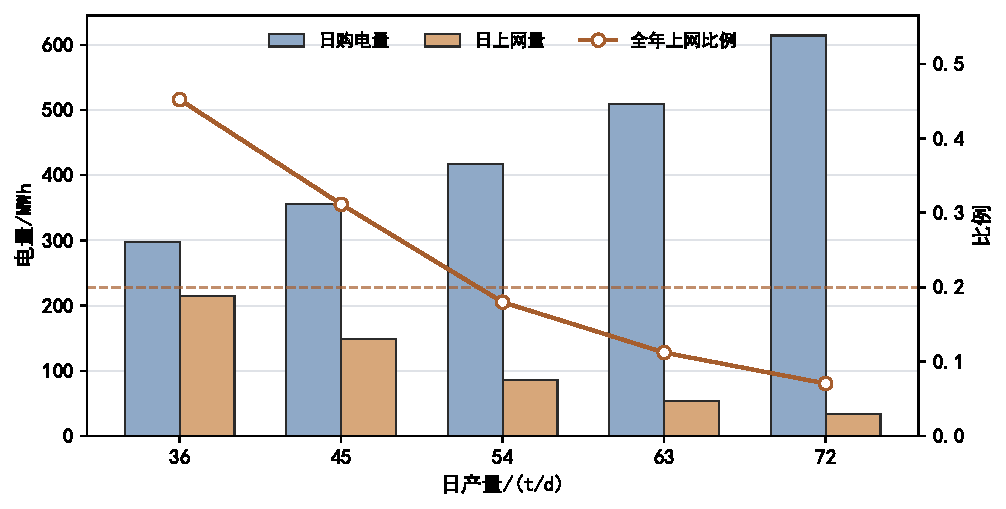
\includegraphics[width=0.85\textwidth]{p2_grid_exchange_distribution.pdf}
  \caption{问题二不同日产量日购电量与日上网量分布}
  \label{fig:p2-grid-exchange-distribution}
\end{figure}

由表~\ref{tab:p2-annual-results} 可见，固定 72、63、54~t/d 运行时，
全年上网比例分别为 0.0705、0.1121、0.1799，均低于 0.20；同时
自发自用比例也保持在 0.8201 以上。但随着日产量降至 45~t/d 和
36~t/d，全年上网比例分别升至 0.3115 和 0.4522，说明装置负荷降低后
新能源就地消纳能力明显下降。另一方面，固定产量的全年吨氨成本随
日产量降低而下降，36~t/d 固定方案为 4493.82~元/t，低于 72~t/d
固定方案的 7182.67~元/t。

若在每个风光场景内独立选择吨氨成本最低的日产量，当前 24 个场景
均选择 36~t/d。因此推荐方案与固定 36~t/d 全年折算结果一致：
年产量为 12960~t，年总净成本为 58\,239\,941.06~元，全年吨氨成本为
4493.82~元/t。对应三项绿电直连指标为
$\Pi_{\mathrm{self}}=0.5478$、
$\Pi_{\mathrm{green}}=0.3369$、
$\Pi_{\mathrm{sell}}=0.4522$；全年 360 天中，全满足天数为 0 天，
部分满足天数为 345 天，全不满足天数为 15 天。推荐方案的吨氨成本
场景分布见图~\ref{fig:p2-annual-unit-cost-distribution}。

\begin{figure}[H]
  \centering
  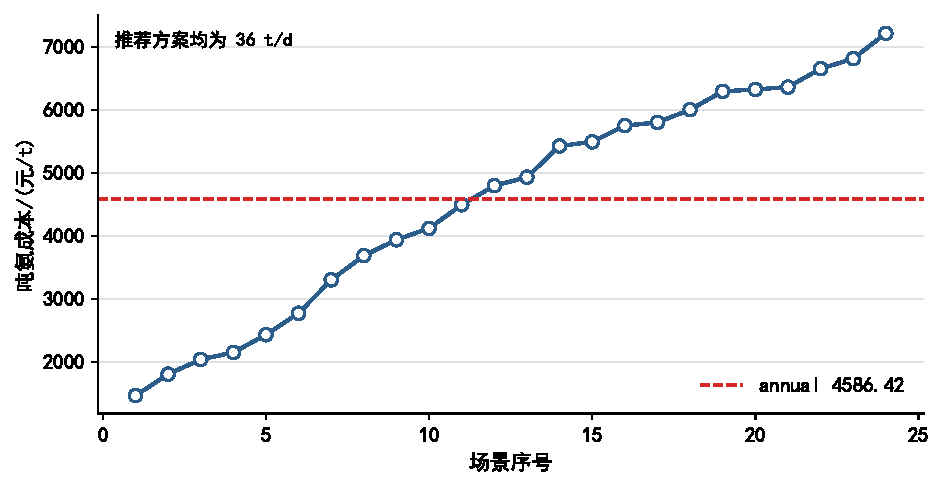
\includegraphics[width=0.82\textwidth]{p2_annual_unit_cost_distribution.pdf}
  \caption{问题二推荐方案吨氨成本场景分布}
  \label{fig:p2-annual-unit-cost-distribution}
\end{figure}

综合典型场景和 24 场景结果可以看出，成本最优与绿电指标最优之间
存在明显冲突。低日产量方案能够把开机时段集中在低净成本小时，
减少高价购电时段的生产负荷，因而吨氨成本最低；但负荷降低后，
风光高出力时段可被园区吸收的电量减少，余电上网比例升高，自发自用
比例下降。高日产量方案则相反，较高的生产负荷能够吸收更多风光
电量，使上网比例下降、绿电指标改善，但需要覆盖更多低出力或高电价
时段，购电支出和设备运行支出随之增加。由此可见，仅以日净成本为
目标的离散开停机策略会偏向低负荷生产，若后续需要同时满足绿电直连
指标，应在目标函数或约束中进一步引入指标达标要求，或进入问题三的
连续功率调节模型提高风光消纳的时间匹配能力。

\section{问题三：基于连续制氨调节的运行分析}

\subsection{模型建立}

问题三仍考虑 24 种风光组合出力场景，但将问题二中的离散开停机调度
推广为连续功率调节。设 $\alpha_{t,s,q}$ 为场景 $s$、目标日产量 $q$
下第 $t$ 个时段电氢氨装置的负荷率。根据题设，装置功率连续可调且下限为
10\%，因此有
\begin{equation}
  0.1 \leq \alpha_{t,s,q} \leq 1,
  \qquad t=1,2,\dots,24.
  \label{eq:p3-alpha-bound}
\end{equation}
与问题二的二元变量 $u_{t,s,q}\in\{0,1\}$ 相比，式~\eqref{eq:p3-alpha-bound}
允许装置在最低负荷和满负荷之间连续变化，从而以更细的功率粒度匹配风光出力。

扩容至 $72~\mathrm{t/d}$ 后，设备满负荷功率沿用问题二参数。连续调节下
各设备功率和产氨速率表示为
\begin{equation}
  P_{t,s,q}^{\mathrm{ALK}}=20\alpha_{t,s,q},\quad
  P_{t,s,q}^{\mathrm{PEM}}=20\alpha_{t,s,q},\quad
  P_{t,s,q}^{\mathrm{NH_3}}=1.5\alpha_{t,s,q},\quad
  m_{t,s,q}^{\mathrm{NH_3}}=3\alpha_{t,s,q}.
  \label{eq:p3-device-power}
\end{equation}
因此，目标日产量约束为
\begin{equation}
  \sum_{t=1}^{24}3\alpha_{t,s,q}\Delta t=q,
  \qquad \Delta t=1~\mathrm{h}.
  \label{eq:p3-production}
\end{equation}
由于每小时至少以 10\% 负荷运行，任一方案均具有 $7.2~\mathrm{t/d}$
的基础产量；其余产量由各时段负荷率的连续增量分配完成。

园区内部用电功率为
\begin{equation}
  P_{t,s,q}^{\mathrm{use}}
  =P_{t,s}^{\mathrm{load}}+41.5\alpha_{t,s,q}.
  \label{eq:p3-use-power}
\end{equation}
购电功率和上网功率继续沿用问题一的功率平衡式~\eqref{eq:power-balance}
以及正负缺额定义式~\eqref{eq:p1-grid-exchange}。同时，为明确同一小时不能
既购电又售电，引入模式变量 $z_{t,s,q}\in\{0,1\}$，并设置
\begin{equation}
  0\leq P_{t,s,q}^{\mathrm{buy}}\leq Mz_{t,s,q},\qquad
  0\leq P_{t,s,q}^{\mathrm{sell}}\leq M(1-z_{t,s,q}),
  \label{eq:p3-grid-exclusive}
\end{equation}
其中 $M$ 为足够大的功率上界。式~\eqref{eq:p3-grid-exclusive} 保证任一时段
内购电和售电至多发生一种。

优化目标仍为最小化日运行净成本：
\begin{equation}
  \min C_{s,q}^{\mathrm{day}},
  \label{eq:p3-objective}
\end{equation}
其中 $C_{s,q}^{\mathrm{day}}$ 的构成与问题二式~\eqref{eq:p2-day-cost}
一致，包括风电和光伏度电成本、设备运维成本、分时购电费用以及余电上网
收入抵扣。吨氨成本继续采用式~\eqref{eq:p2-unit-cost} 的口径计算。
绿电直连指标则沿用问题一式~\eqref{eq:indicators}，并按全满足、部分满足、
全不满足三类统计。

从求解角度看，连续负荷率使各小时的可调空间可在 $0.1$ 到 $1$ 之间连续分配。
当
\begin{equation}
  \alpha_{t,s}^{0}
  =\frac{P_{t,s}^{\mathrm{re}}-P_{t,s}^{\mathrm{load}}}{41.5}
  \label{eq:p3-zero-exchange}
\end{equation}
落在 $[0.1,1]$ 内时，该负荷率对应本时段既不购电也不上网的临界状态。
由于谷电价可能低于余电上网电价，简单地将各小时边际成本独立排序可能会破坏
负荷率的连续路径。本文因此采用带买卖电互斥约束的混合整数线性规划求解，
其目标函数、功率平衡和产量约束均为线性形式，可直接求得连续调节下的全局最优方案。

\subsection{模型求解与结果}

对 24 种风光组合场景和五个目标日产量分别求解连续调节模型，并按每个场景代表
15 天折算全年。表~\ref{tab:p3-annual-result} 给出了固定日产量口径下的全年结果。
与问题二一致，$72~\mathrm{t/d}$ 方案因式~\eqref{eq:p3-production} 要求
$\sum_t\alpha_t=24$，各时段均为满负荷运行，因此与问题二结果相同。
在其他产量下，连续调节可在 24 小时内重新分配负荷率，使生产功率更贴近风光出力。

\begin{table}[H]
  \centering
  \caption{问题三 24 场景全年折算下不同日产量的运行结果}
  \label{tab:p3-annual-result}
  \begin{tabular}{ccccc}
    \toprule
    日产量 & 吨氨成本 & 网购电量 & 上网电量 & 指标天数统计 \\
    (t/d) & (元/t) & (MWh) & (MWh) & 全满足/部分/不满足 \\
    \midrule
    72 & 7228.97 & 221146.80 & 12078.72 & 270/90/0 \\
    63 & 6466.04 & 176326.80 & 12078.72 & 300/60/0 \\
    54 & 5725.68 & 137231.50 & 17803.42 & 240/120/0 \\
    45 & 5082.84 & 109563.64 & 34955.56 & 240/120/0 \\
    36 & 4302.07 & 91060.62 & 61272.54 & 165/195/0 \\
    \bottomrule
  \end{tabular}
\end{table}

从表~\ref{tab:p3-annual-result} 可见，若仅以吨氨成本最低为准，24 个场景下的
推荐方案仍倾向于选择 $36~\mathrm{t/d}$。该方案全年折算制氨量为 12960~t，
总净成本为 55\,754\,817.22~元，吨氨成本为 \textbf{4302.07~元/t}。
其新能源自发自用比例为 $64.24\%$、宽口径总用电绿电比例为 $41.95\%$，
均满足阈值；但新能源上网比例为 $35.76\%$，仍高于 $20\%$ 的要求。
这说明连续调节改善了新能源消纳，但在低日产量下，受总产量需求限制，
仍无法完全吸收高风光场景中的富余电量。

图~\ref{fig:p3-dispatch-example} 给出了代表性场景 $W4\_P1$、日产量
$36~\mathrm{t/d}$ 下的连续调度结果。可以看出，负荷率并非简单取 10\%
或 100\%，而是在不同小时之间连续变化：风光出力较高或购电成本较低时段提高负荷，
风光不足且购电成本较高时段降低负荷，从而同时压低购电量和上网量。

\begin{figure}[H]
  \centering
  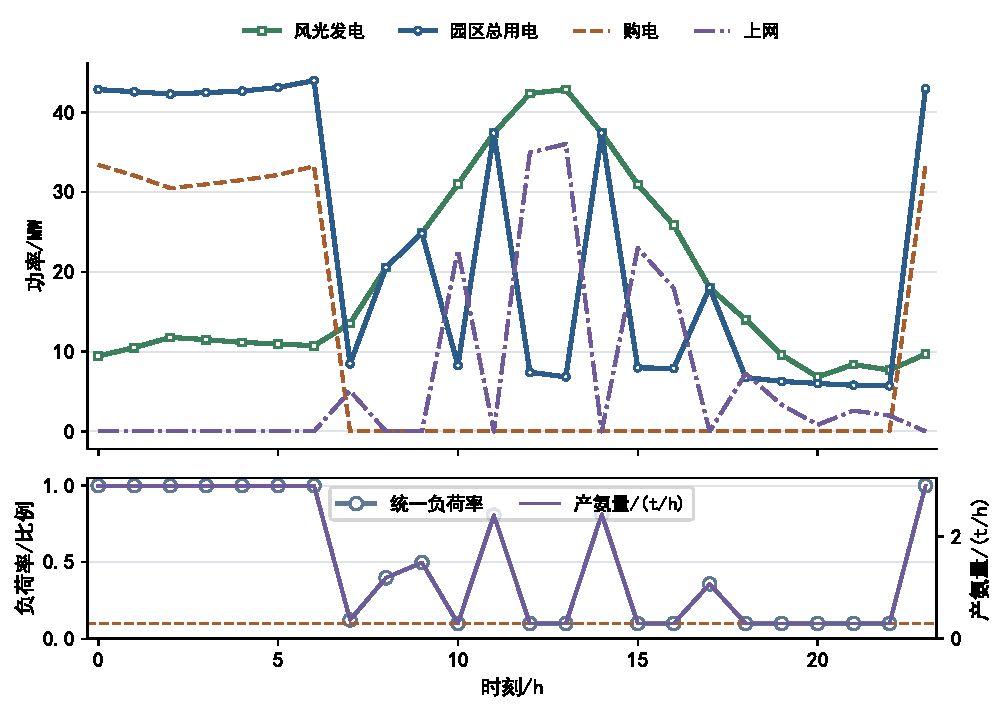
\includegraphics[width=0.88\textwidth]{p3_continuous_schedule.pdf}
  \caption{问题三代表场景下连续负荷率调度与电网交换功率}
  \label{fig:p3-dispatch-example}
\end{figure}

问题三与问题二的全年吨氨成本对比如图~\ref{fig:p3-cost-compare} 所示。
除 $72~\mathrm{t/d}$ 因两种模型均为全天满负荷而结果相同外，其余产量下
连续调节均降低了吨氨成本。其中 $36~\mathrm{t/d}$ 方案的吨氨成本由
4586.42~元/t 降至 4302.07~元/t，下降 284.35~元/t；$45~\mathrm{t/d}$
方案下降 281.55~元/t。成本降低的主要原因在于，连续负荷可以利用离散开停机
难以覆盖的时段，使部分原本上网的新能源转化为内部制氨用电，并减少后续高价
时段的网购电量。

\begin{figure}[H]
  \centering
  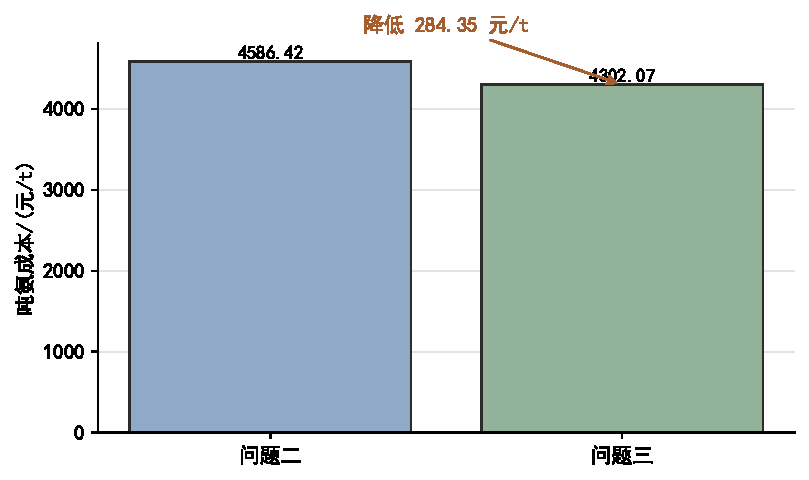
\includegraphics[width=0.82\textwidth]{p3_p2_cost_comparison.pdf}
  \caption{问题二与问题三不同日产量下全年吨氨成本对比}
  \label{fig:p3-cost-compare}
\end{figure}

以成本最低的 $36~\mathrm{t/d}$ 方案为例，问题三相较问题二的全年网购电量
和余电上网量均减少 $1.62\times 10^4~\mathrm{MWh}$。对应三项绿电指标变化如图
~\ref{fig:p3-indicator-compare} 所示：新能源自发自用比例提高 9.46 个百分点，
宽口径总用电绿电比例提高 8.26 个百分点，上网比例降低 9.46 个百分点。
这表明，连续调节的作用并非改变总风光资源，而是改善风光出力与制氨负荷的
时序匹配关系。

\begin{figure}[H]
  \centering
  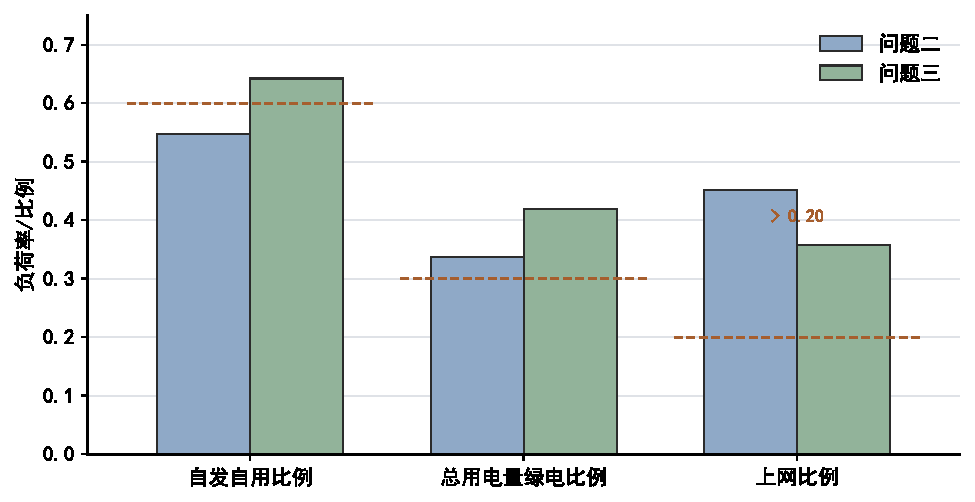
\includegraphics[width=0.78\textwidth]{p3_p2_indicator_comparison.pdf}
  \caption{问题二与问题三成本最低方案的绿电直连指标对比}
  \label{fig:p3-indicator-compare}
\end{figure}

综合来看，连续制氨调节相较离散开停机具有更好的消纳能力和经济性表现：
一方面，低负荷运行下限保证装置全天维持基本生产；另一方面，连续负荷率又允许
模型在新能源富余时段逐步提高功率，而不是被迫在停机和满负荷之间跳变。
因此，问题三模型在大多数产量档位下同时降低了购电量、上网量和吨氨成本。
不过，若要求三项绿电直连指标全部满足，单纯追求最低吨氨成本仍不充分；
例如 $36~\mathrm{t/d}$ 方案虽然成本最低，但上网比例仍超限。若优先考虑指标合规，
$54~\mathrm{t/d}$ 可作为更均衡的方案，其全年吨氨成本为 5725.68~元/t，
自发自用比例为 $89.61\%$、宽口径总用电绿电比例为 $49.76\%$、上网比例为
$10.39\%$，三项指标均满足要求。

\section{问题四：离网运行与储能配置研究}

\subsection{模型建立}

问题四将园区由并网运行转为离网运行，此时外部电网不再补足功率缺额，
园区用能完全受风光发电功率约束。与问题三相同，电氢氨装置运行时功率
连续可调且最低稳定负荷为 10\%；但在离网且风光不足时，装置不能依靠电网
维持最低负荷，因此允许停机。设 $\alpha_{t,s}$ 为场景 $s$ 下第 $t$ 小时
制氨负荷率，则
\begin{equation}
  \alpha_{t,s}=0
  \quad\text{或}\quad
  0.1\leq\alpha_{t,s}\leq1.
  \label{eq:p4-alpha}
\end{equation}
式~\eqref{eq:p4-alpha} 表示：若装置运行，则不得低于 10\% 负荷；
若风光出力连最低稳定负荷也无法支撑，则该时段停机。

无储能时，风光首先满足园区常规负荷，剩余功率用于制氨。记扩容后制氨
系统满负荷用电功率为
\begin{equation}
  P^{\max}=20+20+1.5=41.5~\mathrm{MW}.
  \label{eq:p4-pmax}
\end{equation}
在尽可能利用风光发电的条件下，负荷率按下式确定：
\begin{equation}
  \alpha_{t,s}=
  \begin{cases}
    0, &
    P_{t,s}^{\mathrm{re}}-P_{t,s}^{\mathrm{load}} < 0.1P^{\max},\\[2mm]
    \min\left\{1,\dfrac{P_{t,s}^{\mathrm{re}}-P_{t,s}^{\mathrm{load}}}{P^{\max}}\right\}, &
    P_{t,s}^{\mathrm{re}}-P_{t,s}^{\mathrm{load}} \geq 0.1P^{\max}.
  \end{cases}
  \label{eq:p4-no-storage-alpha}
\end{equation}
对应弃电功率和常规负荷缺额为
\begin{align}
  P_{t,s}^{\mathrm{curtail}}
  &=\max\left\{P_{t,s}^{\mathrm{re}}-P_{t,s}^{\mathrm{load}}
  -P^{\max}\alpha_{t,s},0\right\},\\
  P_{t,s}^{\mathrm{unserved}}
  &=\max\left\{P_{t,s}^{\mathrm{load}}-P_{t,s}^{\mathrm{re}},0\right\}.
  \label{eq:p4-curtail-unserved}
\end{align}
日产氨量为
\begin{equation}
  Q_s=\sum_{t=1}^{24}3\alpha_{t,s}.
  \label{eq:p4-production}
\end{equation}

为量化园区能源自治所需的最小可再生能源装机容量，本文将能源自治界定为基础用电保障能力，
即在全时段离网运行场景下，风光发电出力始终不低于园区常规负荷需求。在此约束框架下，
若风电与光伏装机容量按统一扩容系数 $k$配置，则
\begin{equation}
  k\left(P_{t,s}^{\mathrm{wind}}+P_{t,s}^{\mathrm{pv}}\right)
  \geq P_{t,s}^{\mathrm{load}},\qquad \forall s,t.
  \label{eq:p4-autonomy}
\end{equation}
由此可得最小等比例扩容倍数
\begin{equation}
  k_{\min}=
  \max_{s,t}
  \frac{P_{t,s}^{\mathrm{load}}}{P_{t,s}^{\mathrm{re}}}.
  \label{eq:p4-kmin}
\end{equation}
本模型将“能源自治”界定为保障园区常规负荷的持续供电，不要求全时段满负荷制氨；
否则会使装机规模过度放大，偏离“最小自治容量”的估算目标。

储能参与时，针对无储能结果中的最大弃电场景配置储能。引入充电功率
$P_t^{\mathrm{ch}}$、放电功率 $P_t^{\mathrm{dis}}$、储能电量
$E_t^{\mathrm{ess}}$、储能容量 $E^{\max}$ 和启停变量 $y_t$，有
\begin{equation}
  0.1y_t\leq\alpha_t\leq y_t,\qquad y_t\in\{0,1\}.
  \label{eq:p4-run-status}
\end{equation}
离网功率平衡为
\begin{equation}
  P_t^{\mathrm{re}}+P_t^{\mathrm{dis}}+P_t^{\mathrm{unserved}}
  =
  P_t^{\mathrm{load}}+P^{\max}\alpha_t+P_t^{\mathrm{ch}}+P_t^{\mathrm{curtail}},
  \label{eq:p4-storage-balance}
\end{equation}
储能状态方程为
\begin{equation}
  E_{t+1}^{\mathrm{ess}}
  =(1-\lambda)E_t^{\mathrm{ess}}
  +\eta_cP_t^{\mathrm{ch}}\Delta t
  -\frac{P_t^{\mathrm{dis}}\Delta t}{\eta_d},
  \qquad
  0\leq E_t^{\mathrm{ess}}\leq E^{\max}.
  \label{eq:p4-storage-state}
\end{equation}
其中 $\eta_c=\eta_d=0.9$，$\lambda=0.2\%$。储能配置不单独追求最大消纳，
而是在候选功率--容量组合中同时比较经济折中方案和消纳导向方案：前者以吨氨
成本改善和较小投资为主，后者以最大弃电场景弃电量最小为主。储能投资成本按
使用寿命折算到日成本：
\begin{equation}
  C_{\mathrm{ESS}}^{\mathrm{day}}
  =
  \frac{1000c_{\mathrm{ESS}}^{\mathrm{cap}}E^{\max}}{15\times365}
  +1000c_{\mathrm{ESS}}\sum_tP_t^{\mathrm{dis}}\Delta t,
  \label{eq:p4-storage-cost}
\end{equation}
其中 $E^{\max}$ 单位为 MWh，$c_{\mathrm{ESS}}^{\mathrm{cap}}=1000$ 元/kWh，
储能运维系数 $c_{\mathrm{ESS}}=0.01$ 元/kWh。储能成本按功率、容量和寿命折算
是储能技术经济分析中的常用处理方式~[4]。吨氨成本同时计入风光
度电成本、设备运维、合成氨固定投资折算成本以及储能年化成本。

\subsection{模型求解与结果}

首先计算无储能离网运行结果。原始风光装机下，24 个场景全年折算制氨总量为
9781.56~t，年平均产能利用率为 $37.74\%$，全年弃电量为 14188.67~MWh。
由于个别低出力时段风光甚至不能覆盖常规负荷，全年常规负荷缺额为
8.29~MWh。由式~\eqref{eq:p4-kmin} 得到仅覆盖园区常规负荷的风光等比例
扩容倍数为 $k_{\min}=1.0926$，对应风电装机约为 43.71~MW，光伏装机约为
69.93~MW。若不强制保持风光装机比例，而是在当前 40~MW 风电、64~MW 光伏
基础上最小化新增容量，网格搜索得到的最小自治配置为风电 43.8~MW、光伏
64.0~MW，即仅需新增约 3.8~MW 风电即可覆盖常规负荷。

\begin{figure}[H]
  \centering
  
\includegraphics[width=0.88\textwidth]{p4_offgrid_dispatch_example.pdf}
  \caption{无储能离网条件下代表场景的风光利用与制氨负荷率}
  \label{fig:p4-offgrid-dispatch}
\end{figure}

图~\ref{fig:p4-offgrid-dispatch} 展示了最大弃电场景 $W4\_P1$ 的无储能调度。
当风光出力高于常规负荷和制氨满负荷需求时，制氨负荷率达到 1，剩余功率被弃电；
当风光出力不足以支撑最低稳定负荷时，装置停机。这是离网条件下产能利用率
低于并网情形的重要原因。

无储能结果中，最大弃电场景为 $W4\_P1$。针对该场景进行储能候选配置搜索，
经济折中方案选择 \textbf{5~MW/5~MWh} 储能。该方案下，$W4\_P1$ 场景日产氨量
由 46.19~t 提高至 46.77~t，日弃电量由 177.29~MWh 降至 164.30~MWh，
吨氨成本由 4256.93~元/t 降至 4248.95~元/t。若以最大消纳为目标，
40~MW/160~MWh 储能可将 $W4\_P1$ 弃电量降为 0，并将日产氨量提高至
56.41~t，但吨氨成本升至 4337.38~元/t。因此本文以经济折中方案作为
推荐储能配置。储能充放电和能量状态如图~\ref{fig:p4-storage-dispatch} 所示。

\begin{figure}[H]
  \centering
  
\includegraphics[width=0.88\textwidth]{p4_storage_dispatch.pdf}
  \caption{最大弃电场景下储能参与后的充放电与荷电状态}
  \label{fig:p4-storage-dispatch}
\end{figure}

将该小容量储能用于 24 个场景重新调度，全年折算制氨总量提高至
9969.43~t，年平均产能利用率提高至 $38.46\%$，常规负荷缺额降为 0，
弃电量由 14188.67~MWh 降至 10983.99~MWh。各场景弃电量对比如
图~\ref{fig:p4-curtailment} 所示。结果表明，小容量储能主要承担削减短时
缺额和部分转移富余电量的作用，能够改善能源自治与经济性，但无法完全吸收
所有高峰风光出力。

\begin{figure}[H]
  \centering
  
\includegraphics[width=0.9\textwidth]{p4_curtailment_by_scenario.pdf}
  \caption{无储能与有储能离网运行下各场景日弃电量对比}
  \label{fig:p4-curtailment}
\end{figure}

表~\ref{tab:p4-mode-compare} 比较了联网连续调节、离网无储能和离网有储能三种
运行方式。联网连续调节复用问题三成本最低方案结果。离网无储能的吨氨成本较低，
但存在常规负荷缺额，且全年制氨量明显低于联网方案；配置小容量储能后，常规负荷
缺额被消除，制氨量和吨氨成本均有所改善，但弃电仍然存在。

\begin{table}[H]
  \centering
  \caption{联网与离网运行方式的全年结果对比}
  \label{tab:p4-mode-compare}
  \begin{tabular}{lccc}
    \toprule
    运行方式 & 全年制氨量(t) & 吨氨成本(元/t) & 年产能利用率 \\
    \midrule
    联网连续调节 & 12960.00 & 4302.07 & 50.00\% \\
    离网无储能 & 9781.56 & 4178.99 & 37.74\% \\
    离网有储能 & 9969.43 & 4167.49 & 38.46\% \\
    \bottomrule
  \end{tabular}
\end{table}

\begin{figure}[H]
  \centering
  
\includegraphics[width=0.78\textwidth]{p4_mode_cost_compare.pdf}
  \caption{联网与离网运行方式的吨氨成本和全年制氨量对比}
  \label{fig:p4-mode-compare}
\end{figure}

综合来看，原始风光装机下离网运行可以实现部分能源自治，但受低出力时段制约，
制氨产量和产能利用率下降。小容量储能能够消除常规负荷缺额、减少弃电并略微
降低吨氨成本；大容量储能则可进一步提高风光消纳，但投资成本会削弱经济性。
因此，联网方案在产量稳定性上仍具有优势，而离网储能方案的作用主要体现在提升
能源自治能力和局部风光利用水平。

\section{问题五：高渗透率影响与政策建议}

\subsection{容量渗透率提高对电力系统的利弊}

% TODO

\subsection{推动绿电直连园区发展的政策建议}

% TODO

\section{模型评价与改进}

\subsection{模型优点}

本文模型具有较强的层次性和可解释性。问题一先建立统一功率平衡、绿电指标
和吨氨成本口径，问题二至问题四再依次加入离散开停机、连续负荷率和储能状态
变量，使每一问的变化都能与上一问直接对比。求解方法也与问题结构匹配：
问题二利用开机净成本增量排序，避免枚举大量二元组合；问题三、四采用线性或
混合整数线性模型，便于检查功率平衡、产量约束和购售电互斥约束。所有结果均
保留逐时数据，可追溯到具体场景和时段。

\subsection{模型不足}

模型仍存在一定简化。首先，电解槽和合成氨装置的效率被视为常数，未考虑低负荷
效率变化、启停损耗、爬坡约束和设备寿命折损。其次，24 种风光组合场景按等权
15 天折算全年，不能完全反映真实天气年内相关性。再次，成本中未纳入氨储运、
水耗、检修停机、容量电费和碳交易收益等因素。问题四储能配置以最大弃电场景
为代表，能够体现容量需求上界，但未进一步考虑多日连续阴天和跨日库存。

\subsection{改进方向}

后续可从三方面改进：一是引入更精细的设备运行约束，包括最小开停机时间、
爬坡速率、低负荷效率曲线和制氢--制氨中间库存；二是采用全年逐时风光数据或
概率场景树替代等权日场景，提高年化结果的统计可靠性；三是将绿电直连指标、
辅助服务收益和碳减排收益纳入多目标优化，形成经济性、合规性和系统友好性
之间的 Pareto 权衡方案。

\section{结论}

本节按照题目问题顺序归纳主要结论，突出可直接支撑竞赛论文观点的结果。

\section*{参考文献}
\addcontentsline{toc}{section}{参考文献}

\begin{enumerate}[label={[\arabic*]},leftmargin=2.5em]
  \item 作者，书名，出版地：出版社，出版年，页码.
  \item 作者，论文名，杂志名，卷期号：起止页码，出版年.
  \item 作者，资源标题，网址，访问时间（年月日）.
\end{enumerate}


\clearpage
\appendix
\section{附录}

本文完整源程序、输入数据和中间结果随支撑材料提交。本附录给出关键
求解过程的伪代码，用于说明正文模型与程序实现之间的对应关系。伪代码
只保留主要决策逻辑，不展开数据读取、单位换算和结果写出等工程细节。

\subsection{问题二离散开停机调度}

问题二在给定场景和目标日产量下，只需确定开机小时集合。由于题设未考虑
启停成本、爬坡约束和跨时段库存，日内各小时除开机小时数约束外相互独立，
因此可采用净成本增量排序法求解。

\begin{enumerate}[label=\textbf{步骤~\arabic*.},leftmargin=4em]
  \item 输入风电、光伏、常规负荷和分时电价序列，给定目标日产量 $q$。
  \item 令所需开机小时数 $H=q/3$。
  \item 对每个时段 $t$，分别计算停机状态 $u_t=0$ 与满开状态 $u_t=1$
        下的园区用电功率。
  \item 根据功率缺额计算两种状态下的购电功率和上网功率：
        \[
          P_t^{\mathrm{buy}}=\max(P_t^{\mathrm{use}}-P_t^{\mathrm{re}},0),
          \quad
          P_t^{\mathrm{sell}}=\max(P_t^{\mathrm{re}}-P_t^{\mathrm{use}},0).
        \]
  \item 分别计算两种状态下的风光度电成本、设备运维成本、分时购电成本
        和上网收入抵扣。
  \item 计算该时段由停机转为开机的净成本增量
        $\Delta C_t=C_t(u_t=1)-C_t(u_t=0)$。
  \item 将 24 个时段按 $\Delta C_t$ 从小到大排序，选择前 $H$ 个时段开机，
        其余时段停机。
  \item 根据所得 $u_t$ 序列重新计算逐时功率平衡、三项绿电直连指标和吨氨成本。
\end{enumerate}

\subsection{问题三连续负荷率优化}

问题三将离散开停机变量 $u_t$ 替换为连续负荷率 $\alpha_t$，并设置
$0.1\leq\alpha_t\leq1$。程序中按日场景建立线性约束，并通过购售电互斥
条件避免同一时段同时买电和卖电。

\begin{enumerate}[label=\textbf{步骤~\arabic*.},leftmargin=4em]
  \item 对每个风光组合场景 $s$ 和日产量 $q$，建立变量
        $\alpha_t$、$P_t^{\mathrm{buy}}$、$P_t^{\mathrm{sell}}$ 和互斥变量 $z_t$。
  \item 添加负荷率约束：
        \[
          0.1\leq\alpha_t\leq1,\qquad t=1,2,\dots,24.
        \]
  \item 添加日产量约束：
        \[
          \sum_{t=1}^{24}3\alpha_t=q.
        \]
  \item 由 $P_t^{\mathrm{use}}=P_t^{\mathrm{load}}+41.5\alpha_t$
        建立逐时功率平衡：
        \[
          P_t^{\mathrm{re}}+P_t^{\mathrm{buy}}
          =P_t^{\mathrm{use}}+P_t^{\mathrm{sell}}.
        \]
  \item 通过大 $M$ 约束限制 $P_t^{\mathrm{buy}}$ 与
        $P_t^{\mathrm{sell}}$ 不能同时为正：
        \[
          P_t^{\mathrm{buy}}\leq Mz_t,\qquad
          P_t^{\mathrm{sell}}\leq M(1-z_t).
        \]
  \item 以日运行净成本最小为目标求解，得到连续负荷率序列。
  \item 汇总 24 场景和五个日产量档位的逐时结果，并折算全年成本和绿电指标。
\end{enumerate}

\subsection{问题四离网储能配置}

问题四分为无储能离网调度、能源自治装机估算和储能候选配置比较三部分。
其中储能配置不直接追求最大容量，而是在制氨产量、弃电量和吨氨成本之间
比较经济折中方案。

\begin{enumerate}[label=\textbf{步骤~\arabic*.},leftmargin=4em]
  \item 在无储能条件下，先以风光出力满足常规负荷。
  \item 若剩余功率不低于 $0.1P^{\max}$，则按式~\eqref{eq:p4-no-storage-alpha}
        确定制氨负荷率；否则制氨装置停机。
  \item 对所有场景逐时计算制氨量、弃电量和常规负荷缺额，并识别最大弃电场景。
  \item 根据全时段常规负荷保障条件，计算等比例扩容倍数 $k_{\min}$；
        同时在给定步长下搜索最小新增装机组合。
  \item 对最大弃电场景枚举候选储能功率和容量，建立充电功率、放电功率、
        荷电状态、制氨负荷率和弃电功率之间的日内平衡。
  \item 对每个候选配置求解离网调度，记录日产氨量、弃电量、常规负荷缺额、
        储能年化成本和吨氨成本。
  \item 在候选结果中选择经济折中配置，并将该配置用于 24 场景全年折算。
\end{enumerate}


\end{document}
